\documentclass[12pt]{article}

\usepackage{amsmath}
\usepackage{amssymb}
\usepackage{anyfontsize}
\usepackage[toc,page]{appendix}
\usepackage{array}
\usepackage{booktabs}
\usepackage{caption}
\usepackage{cellspace}
\usepackage{color}
\usepackage{enumerate}
\usepackage{enumitem}
\usepackage{float}
\usepackage{geometry}
\usepackage{graphicx}
\usepackage{newtxtext,newtxmath}
\usepackage{listings}
\usepackage{physics} 
\usepackage{subfigure}
\usepackage{tabularx}

\geometry{
    a4paper,
    total = {170mm, 257mm},
    left = 20mm,
    top = 20mm,
    }

\definecolor{dkgreen}{rgb}{0,0.6,0}
\definecolor{gray}{rgb}{0.5,0.5,0.5}
\definecolor{mauve}{rgb}{0.58,0,0.82}
\lstset{frame = tb,
        language = Python,
        aboveskip = 3mm,
        belowskip = 3mm,
        showstringspaces = False,
        columns = flexible,
        basicstyle = {\small\ttfamily},
        numbers = left,
        numberstyle = \tiny\color{gray},
        keywordstyle = \color{blue},
        commentstyle = \color{dkgreen},
        stringstyle = \color{mauve},
        breaklines = true,
        breakatwhitespace = true,
        tabsize=4}

\renewcommand\lstlistingname{Algorithm}
\captionsetup[lstlisting]{singlelinecheck=false, margin=12pt, labelsep=default, labelfont=default}
%We can also use: labelsep=period or labelsep=spacce, labelfont=default or labelfont=bf


%%%%%%%%%%%%%%%%%%%%%%%%%%%%%%%%%%% Again, Don't change anything Above %%%%%%%%%%%%%%%%%%%%%%%%%%%%%%%%%%%


\begin{document}

\title{\textbf{{\normalsize Computational Physics Lab}\\
                Homework 4}}
\author{108000204\\
        Yuan-Yen Peng\\
        Dept. of Physics, NTHU\\
        Hsinchu, Taiwan}
\date{\today}
\maketitle

\section{Writing Assignments}
    \subsection{Finite difference method for solving 2D Poisson equation}
    The $3 \times 3$ grids with grid space $h$ and the source term $\rho(x,y)$ can be described as:
    \[
        u_{xx} + u_{yy} = \rho(x,y)
    \]
    where the subscripts mean second partial derivatives of the u with $x$ and $y$, respectively. Besides, we annotate $(x,y)$ with $(i,j)$ where $i$ and $j$ are from $0 \sim (3+1)$ (including boundaries, which are $(i,j) = (i,0),\ (i,4),\ (0,j),\text{and}\ (4,j)$), and implement the Euler method for derivative; then we can get:
    \begin{align*}
        &\frac{\partial}{\partial x}\Big( \frac{u_{i,j} - u_{i-1,j}}{h} \Big) + \frac{\partial}{\partial y}\Big( \frac{u_{i,j} - u_{i,j-1}}{h} \Big) = \rho(x,y) \\
        \Rightarrow &\frac{1}{h} \Big( \frac{u_{i+1,j} - u_{i,j}}{h} - \frac{u_{i,j} - u_{i-1,j}}{h} \Big) + \frac{1}{h} \Big( \frac{u_{i,j+1} - u_{i,j}}{h} - \frac{u_{i,j} - u_{i,j-1}}{h} \Big) = \rho(x,y) \\
        \Rightarrow &\big( u_{i+1,j} - 2u_{i,j} + u_{i-1,j} \big) + \big( u_{i,j+1} - 2u_{i,j} + u_{i,j-1} \big) = \rho(x,y) h^{2} \\
        \Rightarrow&\ 4_{i,j} - u_{i-1,j} - u_{i+1,j} - u_{i,j-1} - u_{i,j+1} = \rho(x,y) h^{2} \tag{I}\label{A}
    \end{align*}
    In the wake of knowing the general form of the solution, we apply the boundary conditions; here boundaries are all zeros (i.e., $u_{0,j},\ u_{i,0},\ u_{4,j},\ \text{and}\ u_{i,4} = 0$). Exploiting all $i$ and $j$, we can get LHS of eq.(\ref{A}) in the matrix form $\mathbf{A}$ and RHS in the vector form $\mathbf{b}$ with source term $g_{ij}$ which represents the splitting of the source function $\rho(x,y)$:
    \[
        \mathbf{A} = 
        \begin{bmatrix}
            \begin{bmatrix}
                4  & -1 & 0 \\
                -1 & 4  & -1\\
                0  & -1 & 4 \\
            \end{bmatrix}
            &
            \begin{bmatrix}
                -1 & 0  & 0 \\
                0  & -1 & 0 \\
                0  & 0  & -1\\
            \end{bmatrix}
            &
            \begin{bmatrix}
                0 & 0 & 0 \\
                0 & 0 & 0 \\
                0 & 0 & 0\\
            \end{bmatrix}
            \\
            \\
            \begin{bmatrix}
                -1 & 0  & 0 \\
                0  & -1 & 0 \\
                0  & 0  & -1\\
            \end{bmatrix}
            &
            \begin{bmatrix}
                4  & -1 & 0 \\
                -1 & 4  & -1\\
                0  & -1 & 4 \\
            \end{bmatrix}
            &
            \begin{bmatrix}
                -1 & 0  & 0 \\
                0  & -1 & 0 \\
                0  & 0  & -1\\
            \end{bmatrix}
            \\
            \\
            \begin{bmatrix}
                0 & 0 & 0 \\
                0 & 0 & 0 \\
                0 & 0 & 0\\
            \end{bmatrix}
            &
            \begin{bmatrix}
                -1 & 0  & 0 \\
                0  & -1 & 0 \\
                0  & 0  & -1\\
            \end{bmatrix}
            &
            \begin{bmatrix}
                4  & -1 & 0 \\
                -1 & 4  & -1\\
                0  & -1 & 4 \\
            \end{bmatrix}
        \end{bmatrix}
    \]
    and 
    \[
        \mathbf{b} = -h^{2}
        \begin{bmatrix}
            g_{11}\\
            g_{12}\\
            g_{13}\\
            \\
            g_{21}\\
            g_{22}\\
            g_{23}\\
            \\
            g_{31}\\
            g_{32}\\
            g_{33}\\
        \end{bmatrix}
    \]

    \section{Programming Assignments}
    \subsection{$\rho_{22} = 1$ and else are zeros}
    Homework's figure in the last problem is $4 \times 4$, but the question asks the $3 \times 3$ matrix. Thus, I generate the two results in Figure\ref{q1}, the left one uses the definition of the left bottom corner, and the other (right) implements the center of the grid as a benchmark.

    \begin{figure}[H]
        \centering 
        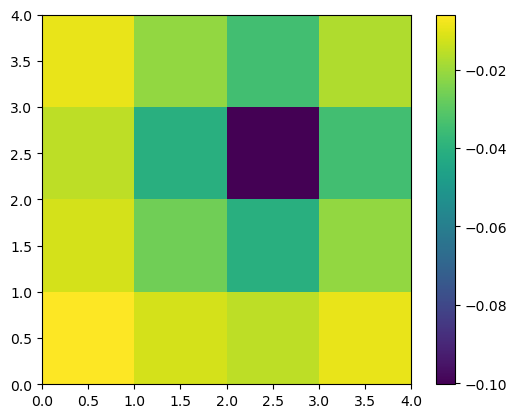
\includegraphics[width = 0.45\textwidth]{./fig/1.1.png}
        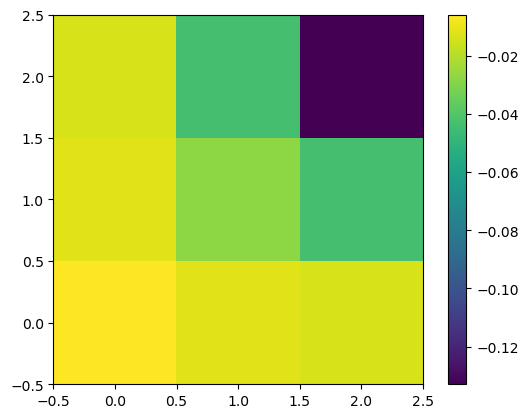
\includegraphics[width = 0.45\textwidth]{./fig/1.2.png} 
        \caption{The left is the $4 \times 4$ grid; the right is the $3 \times 3$ grid. Both of them are with the source $\rho_{22} = 1$ and the others are zeros.}\label{q1}
    \end{figure}

    \subsection{2D Poisson's equation with a given source with periodic boindary}
    In this subsection, we exploit the finite difference method with the sparse matrix to solve the equation:
    \[
        \rho(x,y) = e^{-{5 \over 4} r^{2}_{1}} + {3 \over 2} \times e^{-r^{2}_{2}}
    \]
    with the domain $\mathscr{D}\big\{ [-5 < x < 5] \times [-5 < y < 5] \big\}$ in the $128 \times 128$ grid.

    \begin{figure}[H]
        \centering
        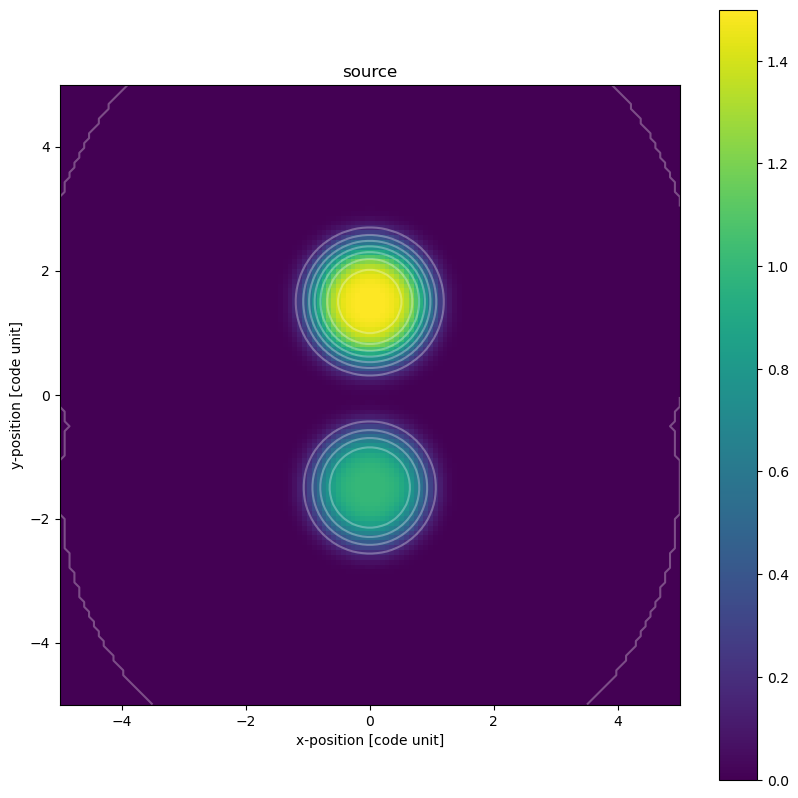
\includegraphics[width = 0.45\textwidth]{./fig/2.1.png}
        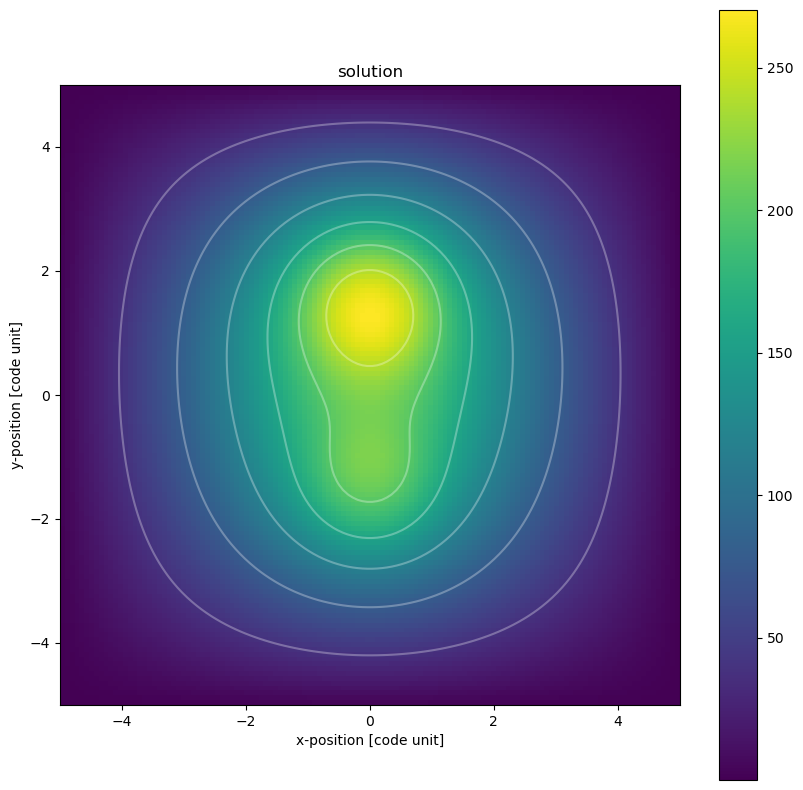
\includegraphics[width = 0.45\textwidth]{./fig/2.2.png}
        \caption{The left is the source function with the scheme with periodic boundary; the right is the solution of the corresponding potential for this Poisson's equation also with the periodic boundary exploiting the sparse matrix method. Moreover, this ``periodic boundary'' will be updated in each run during finite difference algorithm execution.}
    \end{figure}

    \subsection{Error convergence comparison between different algorithms}
    We utilize three different methods learned in the lecture to investigate the error convergence of this Poisson's equation. The first method we used is the Jacobi method and the second is the Gauss-Seidel method, and the last method is the successive over-relaxation method with $w = 1.2,\ 1,5,\text{and}\ 2.0$. However, in SOR (successive over-relaxation method), it might be ``diverge'', so we plot two schemes to research the convergence rate, one is all converge and the other is one of them diverge, please see in Figure\ref{q3}.

    \begin{figure}[H]
        \centering
        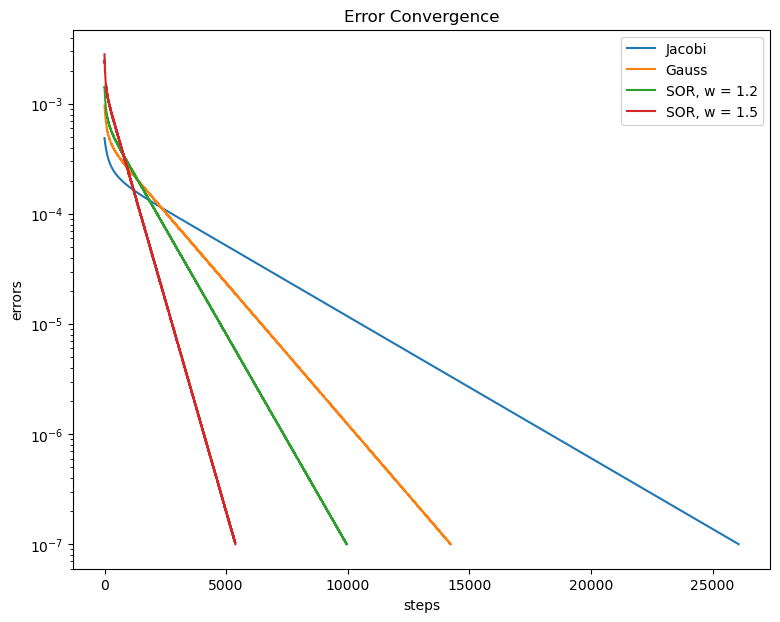
\includegraphics[width = 0.45\textwidth]{./fig/3.1.png}
        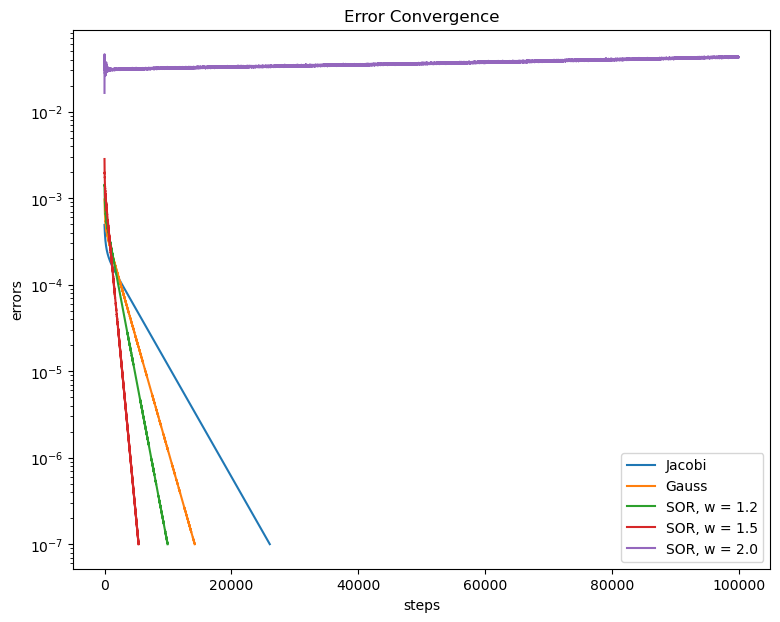
\includegraphics[width = 0.45\textwidth]{./fig/3.2.png}
        \caption{These two figures have the log-scale y-axis; normal scale x-axis. The left is all of methods are converged; the right scheme is the one diverge situation ($w = 2.0$).}\label{q3}
    \end{figure}

    It is manifestly that the Jacobi method is the slowest one and then is the Gauss-Seidel method, and the fastest is the SOR method. In this scenario, although SOR is the fastest when $w = 1.5$, it will diverge with $w = 2.0$ (Figure\ref{q3}-right)! The fastest (SOR with $w = 1.5$) is approximately 4.5 times faster than the slowest (Jacobi) as the error tolerence is $\sim 10^{-6}$.


\section{Codes}
    All the codes are transferred from jupyterlab or python codes; hence, if you want to re-run them, please see the source code in the attached files or my GitHub repository:

    {\centerline{\ttfamily <https://github.com/gary20000915/Comphyslab-HW4.git>}}

    \subsection{{\ttfamily\ particles.py}}
        \begin{lstlisting}[language={Python}]
        
        \end{lstlisting}

\end{document}